\documentclass[conference]{IEEEtran}
\IEEEoverridecommandlockouts
% The preceding line is only needed to identify funding in the first footnote. If that is unneeded, please comment it out.
\usepackage{cite}
\usepackage{amsmath,amssymb,amsfonts}
\usepackage{algorithmic}
\usepackage{graphicx}
\usepackage{textcomp}
\usepackage{xcolor}
\usepackage{tabularx}
\usepackage{multirow}
\usepackage{graphics} % for pdf, bitmapped graphics files
\usepackage{subfig}
\usepackage{subcaption}
\usepackage{hyperref}
\usepackage{academicons}
\usepackage{xcolor}
\usepackage{listings}
\usepackage{tabularx} % Asegúrate de incluir este paquete

\usepackage{tikz}
\usetikzlibrary{shapes.geometric, arrows}

\usetikzlibrary{shapes.geometric, arrows}

\tikzstyle{startstop} = [rectangle, rounded corners, minimum width=3cm, minimum height=1cm,text centered, draw=black, fill=red!30]
\tikzstyle{process} = [rectangle, minimum width=3cm, minimum height=1cm, text centered, draw=black, fill=blue!30]
\tikzstyle{arrow} = [thick,->,>=stealth]


\def\BibTeX{{\rm B\kern-.05em{\sc i\kern-.025em b}\kern-.08em
		T\kern-.1667em\lower.7ex\hbox{E}\kern-.125emX}}

% Color Enlace
\definecolor{colorEnlace}{RGB}{0, 0, 0}
\hypersetup{
	colorlinks=true,
	linkcolor=colorEnlace,
	citecolor=colorEnlace,
	urlcolor=colorEnlace,
	pdfauthor={Davis Bremdow Salazar Roa},
	pdftitle={Transmisión TDM - Telecomunicaciones II}
}
\lstset{
	language=C,
	basicstyle=\ttfamily\small,
	keywordstyle=\color{blue},
	stringstyle=\color{red},
	commentstyle=\color{green!60!black},
	showstringspaces=false,
	numbers=left,
	numberstyle=\tiny\color{gray},
	frame=none,
	breaklines=true,
	tabsize=1
}

% Control 
\usepackage{amsmath}
\begin{document}
	
	\title{Transmisión de datos mediante TDM}
	\author{
		\makebox[\textwidth][c]{\large\textbf{Universidad Nacional de San Antonio Abad del Cusco}}\\
		\makebox[\textwidth][c]{\normalsize\textit{Escuela profesional de Ingeniería Electrónica}}\\
		\makebox[\textwidth][c]{\normalsize\textit{Telecomunicaciones II}}\\
		\and
		\IEEEauthorblockN{Alexander Palomino Lopez}
		\IEEEauthorblockA{Ingeniero Electrónico \\
			Cusco, Perú \\
			alexander.palomino@unsaac.edu.pe}
		\and
		\IEEEauthorblockN{Davis Bremdow Salazar Roa - 200353}
		\IEEEauthorblockA{Estudiante de Ingeniería Electrónica \\
			Cusco, Perú \\
			200353@unsaac.edu.pe}
	}
	
	\maketitle
	\begin{abstract}
		
	\end{abstract}
	\begin{IEEEkeywords}
		Transmisión de datos, Ancho de banda, PCM, TDM, sincronización de canal
	\end{IEEEkeywords}
	
	\section{Introducción}
	
	La Multiplexación por División de Tiempo (TDM, por sus siglas en inglés) es una técnica fundamental en los sistemas de telecomunicaciones modernos, ya que permite la transmisión eficiente de múltiples señales digitales o analógicas a través de un mismo canal físico. Su importancia radica en la optimización del uso del ancho de banda disponible, reduciendo costos de infraestructura y aumentando la capacidad de los sistemas de comunicación.
	
	El principio de la TDM se basa en asignar intervalos de tiempo específicos a cada señal dentro de un marco de transmisión, garantizando que todas compartan el mismo medio sin interferencias. Esta característica la convierte en una herramienta esencial en redes de telefonía, sistemas satelitales, transmisión de datos en fibra óptica y en aplicaciones de comunicación digital como la televisión digital y los servicios de internet de alta velocidad.
	
	Gracias a la TDM, es posible integrar diferentes tipos de información —voz, video y datos— en un mismo canal de forma organizada, manteniendo la calidad del servicio y facilitando la escalabilidad de las redes. En consecuencia, la TDM no solo representa una solución técnica eficiente, sino también una base clave para el desarrollo de sistemas de comunicación modernos que requieren alta velocidad, confiabilidad y capacidad de integración.
	
	\section{Esquema general}
	
	La Multiplexación por División de Tiempo permite la optimización en la cantidad de canales a usar para la trasmisión de datos digitales optimizando así el ancho de banda necesario para transmitir información de diferentes fuentes, en la figura \ref{fig:pcm-blocks} se muestra un esquema general para la transmisión de datos mediante este esquema.
	
	\begin{figure}[h]
		\centering
		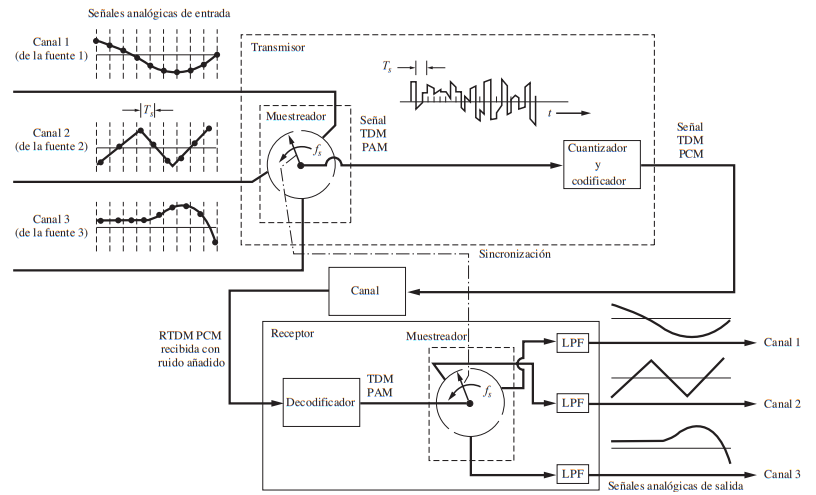
\includegraphics[width=0.5\textwidth]{media/pcm-blocks}
		\caption{Diagrama de bloques - TDM}
		\label{fig:pcm-blocks}
	\end{figure}
	
	Y en la cual se pueden apreciar 6 canales siendo 3 ellos de origen analógico y los restantes digitales, destacando que la transmisión se realiza de forma digital, en esta primera etapa es necesario transformar cada señal continua en una PCM ó  codificación de los pulsos discretos haciendo uso de la frecuencia de muestreo adecuada para cada canal (para definir la frecuencia el teorema de Nyquist puede servir como punto de partida), con cada canal ya digitalizado el bloque de \textbf{SONDEO} se encarga de realizar la mezcla de todas las fuente de información para su transmisión dividiendo este resultado en intervalos de tiempo correspondiente a cada fuente mientras que en el lado del receptor para recuperar cada señal se realiza el proceso inverso.
	
	\section{Sincronización}
	
	La optimización de un canal para el transmisión de información requiere ciertos parámetros de control entre los cuales se puede destacar por su importancia la señal de conmutación o de sincronización la cual es la encargada de generar los bloques de información o slots conformados a partir de las diferentes fuentes que conforman el bloque general TDM que consiste principalmente en la generación de paquetes de información espaciados temporalmente y reconstruidos en función al mismo principio de división en tiempo.
	
	Por lo tanto al requerirse en ambas etapa (envio y recepción) es necesario considerar que la señal de sincronización que actua al mismo tiempo de frecuencia de muestreo (en caso de contar con señales analógicas) debe ser la misma en ambos extremos de un enlace de comunicación digital por lo tanto para su despliegue se desarrollando 2 formas de poder \textbf{sincronizar} este recurso tan relevante.
	
	\begin{itemize}
		\item Sincronización de canal
		\item Sincronización mediante ---
	\end{itemize}
	
	Siendo para el presente caso el empleo de una sincronización de canal en la cual se hace de un canal externo para sincronizar las señales de conmutación permitiendo recuperar de forma efectiva las señales multiplexadas en el tiempo.
	
	
	\section{Simulación}
	\section{Código generado}
	\section{Resultados}
	
	\bibliographystyle{IEEEtran}
	\bibliography{biblio}
\end{document}